\documentclass{beamer}
\usetheme{CambridgeUS}
\usecolortheme{seahorse}

\graphicspath{{media/}}
\usepackage{amssymb}
\usepackage{graphicx}
\usepackage{subcaption}
\usepackage{chronology}

\AtBeginSection[]
{
  \begin{frame}<beamer>
    \tableofcontents[currentsection]
  \end{frame}
}


%                          Information for the Title Page
%
\title[Backpropagation and training neural networks]{
	\Large Deep Feedforward Networks~\cite{Goodfellow-et-al-2016} \\
	[5mm] \normalsize Sarntal Ferienakademie -- Course 10 \\
	Computational Medical Imaging
}
\author{Rayen Manai}


% uncomment appropriate affiliation
\institute[]{
    TU München\\
}
\date{17.09.2023 -- 29.09.2023}
\titlegraphic{%
	\vspace{5mm}%
	
\includegraphics[height=7mm]{FAU_TechFak_Q_RGB_black}%
	\hspace{10mm}%
	
\includegraphics[height=7mm]{tum_logo}%
	\hspace{10mm}%
	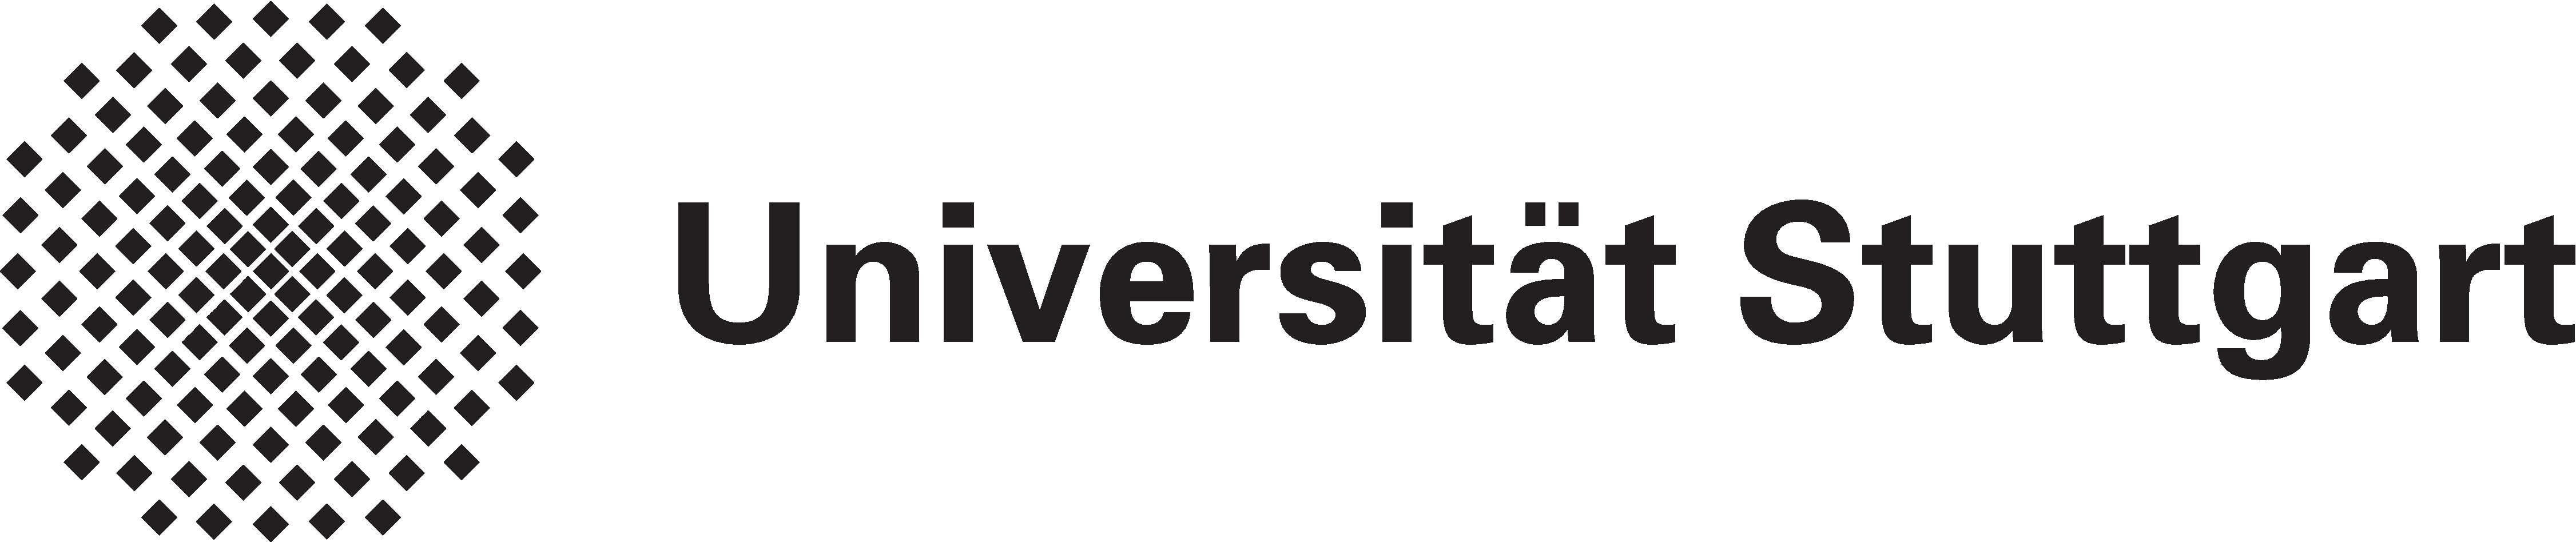
\includegraphics[height=7mm]{stuttgart_logo}%
}


%                                Beginning of the document 
%
\begin{document}
\begin{frame}
	\titlepage
\end{frame}

\begin{frame}
	\frametitle{Outline}
	\tableofcontents
\end{frame}

%---------------------------------------------------------------------- SLIDE -
\section{Introduction}
\begin{frame}
 \frametitle{What do we expect from deep learning?}
	\begin{itemize}
		\item Solve tasks that are easy for people to perform but hard for people to describe formally 
		\item problems that we solve intuitively, like recognizing spoken words or faces in images.
		\item Goal: allow computers to learn from experience and understand the world in terms of a hierarchy of concepts
		\item a graph showing how these concepts are built $\rightarrow$ a deep graph $\rightarrow$ deep Learning
		\item the ability to acquire knowledge, by extracting patterns from raw data
	\end{itemize}

\end{frame}


\section{What is a deep feedforward network?}
\begin{frame}
\begin{itemize}
	\item Deep feedforward network = feedforward neural netwrok = multilayer perceptrons (MLPs)
	\item essential deep learning model
	\item Goal: approximate some function $f\ast$
	\item for example: for a classifier $y = f*(x) \rightarrow$ approxiamte it with $y = f(x;\theta)$
	\item feedfoward? $x \rightarrow$ intermidiate computations $\rightarrow $ output y
	\item networks? represented by composing together many different functions
	\item The model is a directed acyclic graph: how the functions are compoded together, layers, depth, width, hidden layers, units
\end{itemize}
\end{frame}
\begin{frame}
	\frametitle{Overview}
	\center
	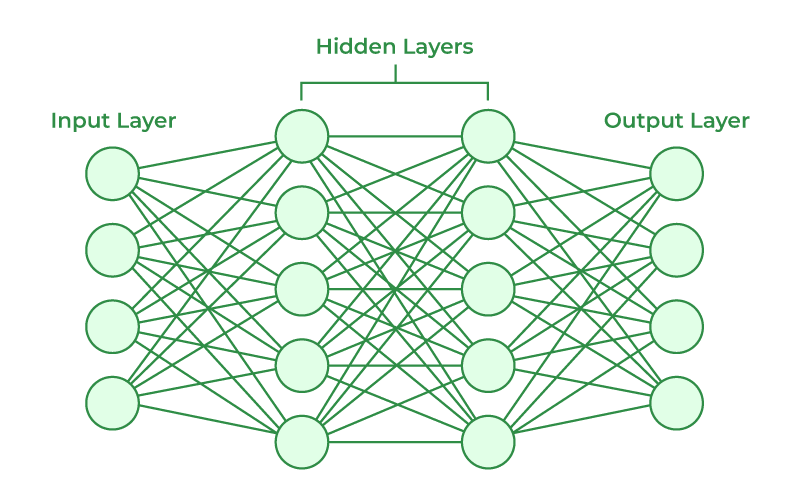
\includegraphics[width= 100mm, height = 70mm]{Neural-Networks-Architecture.png}
\end{frame}
\begin{frame}
	\center
	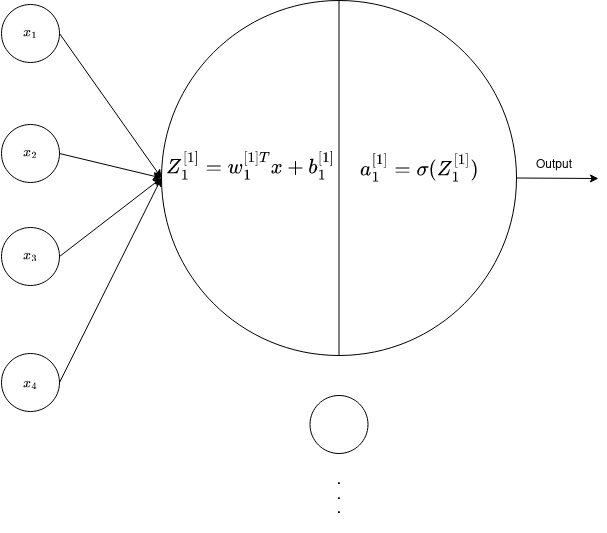
\includegraphics[width = 100mm, height= 70mm]{single_neuron.png}
\end{frame}
\begin{frame}
	\frametitle{Recap: Linear Regression}
	\begin{itemize}
		\item a linear approach used to fit a predective model to an observed data set
		\item error reduction in prediction
		\item often fitted using the least squares approach
	\end{itemize}
	\center 
	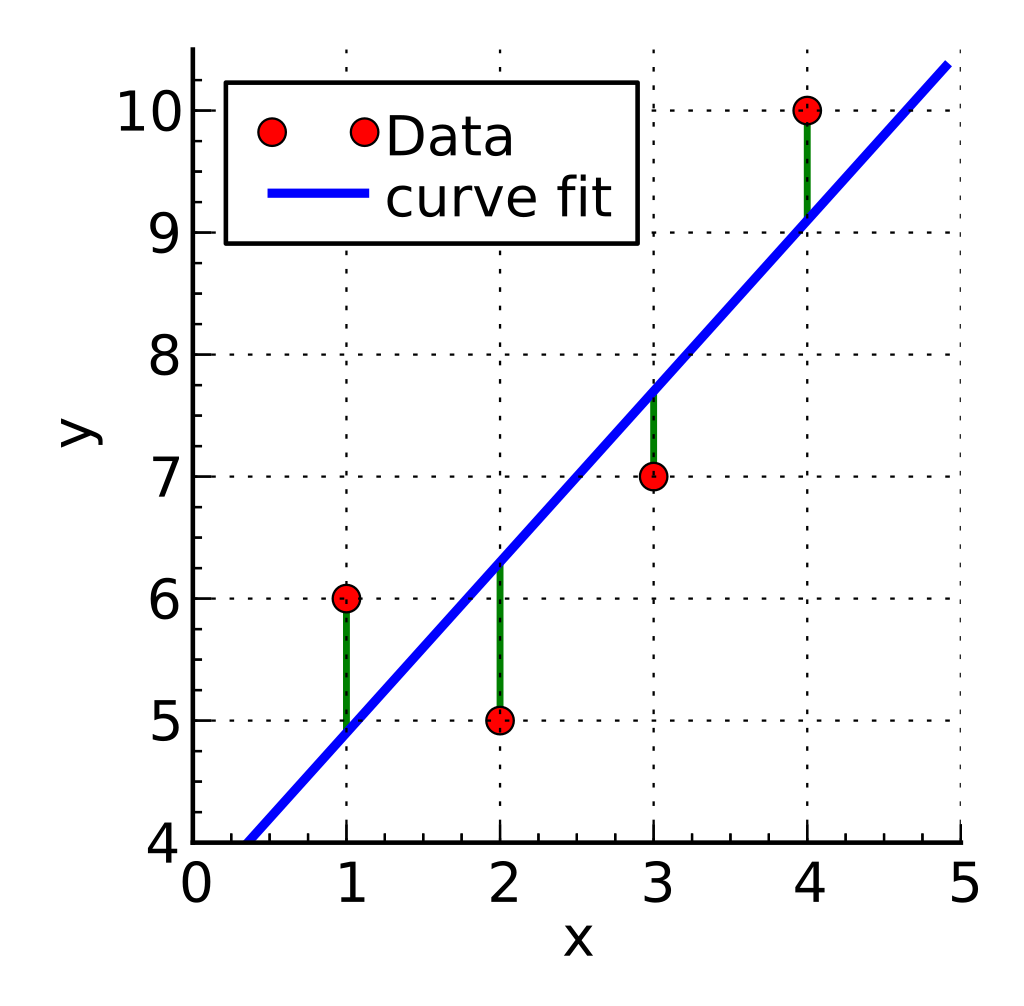
\includegraphics[width= 80mm, height= 45mm]{linear_least_squares.png}
\end{frame}
\begin{frame}
	\frametitle{Example: Learning XOR}
	\center
	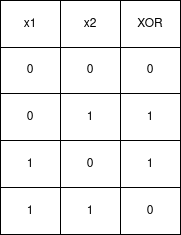
\includegraphics[width= 30mm , height = 30mm]{xor_tabel.png}
	\begin{itemize}
		\item The XOR function provides the target function $y = f\ast(x)$that we want to learn.
		\item Our model provides a function $y = f(x \; \theta)$ and
our learning algorithm will adapt the parameters $\theta $ to make
$f$ as similar as possible to $f\ast$
\item Train the model on the four points $\mathbf{X}= \{ [0,0]^T , [0,1]^T , [1,0]^T, [1,1]^T  \}$	
	\end{itemize}
\end{frame}
\begin{frame}
	\frametitle{First choice: Linear Model}
	\begin{itemize}
\item Treat the problem as a regression problem and use a mean squared error loss function $$ J(\theta) = \frac{1}{4} \sum_{x \in X}{(f\ast(x) - f(x; \theta))^2}$$
		\item we chose a linear model: $$ f(x, w, b) = x^Tw + b$$
		\item we minimize $(\theta)$ with respect to $w$ and $b$ 
		\item $\rightarrow$ we obtain $w = 0$ and $b= 0.5$ 
		\item the linear model simply outputs 0.5 everywhere
	\end{itemize}
	\center 
	Why does this happen?	
\end{frame}

\begin{frame}
	\frametitle{Explanation}
	\begin{itemize}
		\item A linear model is not able to represent the XOR function
		\item XOR is not linearly seperable
	\end{itemize}
	\center 
	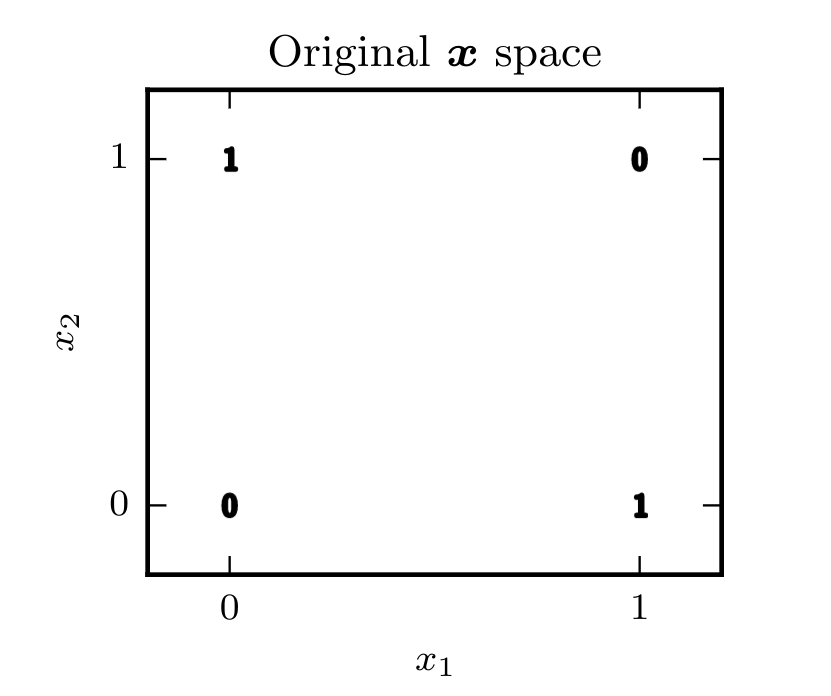
\includegraphics[width = 80 mm, height = 60mm]{xor_graph1.png}
	
\end{frame}
\begin{frame}
	\frametitle{Second choice: different feature space}
	\begin{itemize}
		\item a simple feedforward network with one hidden layer (containing two hidden units)
		\item the network now contains two function chained together
			$$ h= f^{(1)}(x, W, c)$$ and $$ y = f^{(2)}(h, w, b)$$
	\end{itemize}
	\center 
	What function should $f^{(1)}$ compute? Can it be linear?
\end{frame}
\begin{frame}
\begin{itemize}
	\item No, the feedforward netwrok as whole would remain a linear function of its input
	\item $\rightarrow$ we use an affine transformation controlled by learned parameters, followed by a fixed nonlinear function called activation function $$h= g(W^Tx + b)$$
	\item $W$: provides the weights of a linear transformation
	\item $b$: provides the biases
\end{itemize}
\end{frame}
\begin{frame}
	\frametitle{Network Diagram}
	\center 
	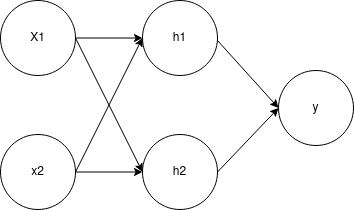
\includegraphics[width= 60mm, height=40mm]{xor_nn.png}	
\end{frame}
\begin{frame}
	\frametitle{Solving XOR}
	\begin{itemize}
		\item The complete Newtork: $f(x, W, c, w, b) = w^Tmax\{0,W^Tx + c\} + b$
		\item We can specify a solution:
			$$ W = \begin{bmatrix} 1 & 1\\
						1 & 1
				\end{bmatrix} , c = \begin{bmatrix}
0\\
-1 
\end{bmatrix} , w = \begin{bmatrix}
1\\
-2
\end{bmatrix}, b = 0$$
\item $\mathbf{X}$ the design matrix containing all four inputs with one example per Column: $\mathbf{X} = \begin{bmatrix}
		0 & 1 & 0 & 1\\
	0 & 0 & 1 & 1 \\
\end{bmatrix}$
	\end{itemize}	
\end{frame}
\begin{frame}
	\frametitle{Let's compute it: }
	\begin{itemize}
		\item $ W^TX + c = \begin{bmatrix} 1 & 1\\
						1 & 1
				\end{bmatrix} .   \begin{bmatrix}
		0 & 1 & 0 & 1\\
	0 & 0 & 1 & 1 \\
\end{bmatrix} + c = \begin{bmatrix}
0\\
-1 
\end{bmatrix} =  \begin{bmatrix}
		0 & 1 & 1 & 2\\
	-1 & 0 & 0 & 1 \\
\end{bmatrix} $
\item Activations of the first layer: the rectified Linear Transformations:
	$$ max\{0,W^TX + c\} =\begin{bmatrix}
		0 & 1 & 1 & 2\\
	0 & 0 & 0 & 1 \\
\end{bmatrix}  $$
\item Activations of the second layer (output): 
	$$  w^Tmax\{0,W^Tx + c\} + b = \begin{bmatrix}
		1 & -2\\
\end{bmatrix}. \begin{bmatrix}
		0 & 1 & 1 & 2\\
	0 & 0 & 0 & 1 \\
\end{bmatrix} = \begin{bmatrix}
		0 & 1 & 1 & 0\\
\end{bmatrix}$$
	\end{itemize}
	$\rightarrow$ the correct answer for every example
\end{frame}
\begin{frame}
	\frametitle{What have we changed?}
	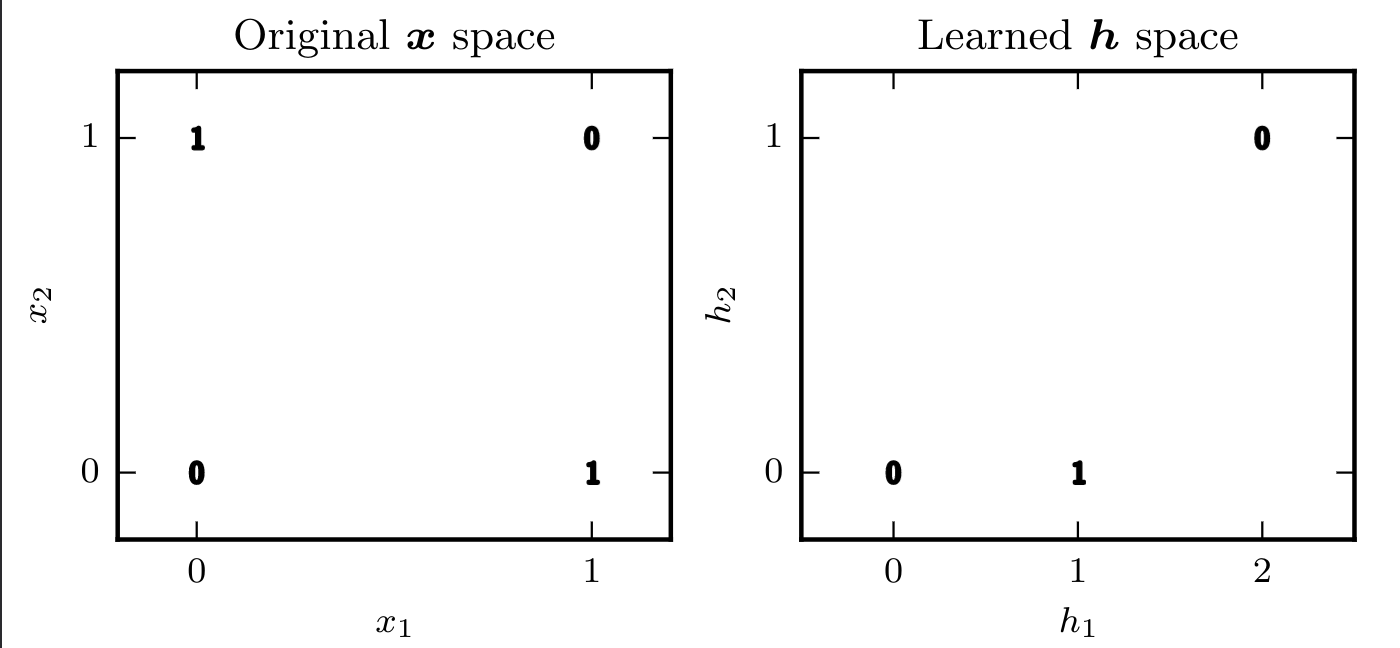
\includegraphics[width=125mm,height =70mm]{xor_graph2.png}
	
\end{frame}



\section{Gradient Based Learning}
\begin{frame}
\begin{itemize}
	\item The nonlinearity of a neural network causes most interesting loss functions to become nonconvex
	\item For feedforward neural networks, it is important to
initialize all weights to small random values. 
\item we will describe how to obtain the gradient using the back-propagation
algorithm and modern generalizations of the back-propagation algorithm
\item we must choose a cost function, and we must choose how to represent the output of the model
	
\end{itemize}
\end{frame}

\subsection{Cost Functions}
\begin{frame}
	\begin{itemize}
		\item An important aspect of the design of a deep neural network is the choice of the cost function
		\item In general, the model defines a distribution $p(y|x;\theta)$ and we use the principle of maximum likelihood
		\item $\rightarrow$ The cross-entropy between the training data and the model's predictions as the cost function.
		\item The total cost function combines a cost function with a regularization term
	\end{itemize}
\end{frame}
\begin{frame}
	\frametitle{Learning Conditional Distributions with Maximum Likelihood}
	\begin{itemize}
		\item the cost function is simply the negative log-likelihood, equivalently described as the cross-entropy between the training data and the model distribution.
			$$ J(\theta)= -\mathbb{E}_{x,y\sim \hat{p}_{data}\log p_{model}}(y|x)$$
		\item used to evaluate the performance of a model's predicted probability distribution against the true distribution of the data
		\item In the context of binary classification, where $y$ is the true probablity and $\hat{y}$ the predicted probability:
			$$ J = -(y\log \hat{y} + (1-y) \log (1- \hat{y}))$$
	\end{itemize}	
\end{frame}
\begin{frame}
	\frametitle{Example Binary Classification:}
	\begin{itemize}
\item In the context of binary classification, where $y$ is the true probablity and $\hat{y}$ the predicted probability:
			$$ J = -(y\log \hat{y} + (1-y) \log (1- \hat{y}))$$
		\item $y = 1 \rightarrow J =-(y\log \hat{y}) \rightarrow \hat{y}$ large, closer to 1
		\item $y = 0 \rightarrow J =-\log (1-\hat{y}) \rightarrow 1- \hat{y}$ large, $\hat{y}$ closer to 0



		
	\end{itemize}
	
\end{frame}

\subsection{Output Units}
\begin{frame}
	\begin{itemize}
		\item The choice of cost function is tightly coupled with the choice of output unit
		\item The choice of how to represent the output then determines the form of the cross-entropy function
		\item Linear Units for Gaussian Output: 
			$$ \hat{y}= W^Th + b $$
		\item Sigmoid Units: 
			$$\hat{y}=\sigma (w^Th+b) $$
		\item Softmax Units:
		
	\end{itemize}
\end{frame}

\section{Hidden Units}
\begin{frame}
	\begin{itemize}
		\item So far, design choices for neural networks that are common to most parametric machine learning models trained with gradient-based optimization
		\item Now: how to choose the type of hidden unit to use in the hidden layers of the model
		\item  extremely active area of research and does not
yet have many definitive guiding theoretical principles
\item Rectified linear units are an excellent default choice of hidden unit
\item It can be difficult to determine when to use which kind
\item The design process consists of trial and error
\item Some of the hidden units included in this list are not actually differentiable at all input points
\item Hidden units that are not differentiable are usually nondifferentiable at only a small number of points.
\item in practice one can safely disregard the nondifferentiability of the hidden unit activation functions described below
	\end{itemize}
\end{frame}
\begin{frame}
	\frametitle{Role of hidden units: }
	\begin{itemize}
		\item accept a vector of inputs $x$
		\item compute an affine transformation: $z = W^Tx + b$
	\end{itemize}
	
\end{frame}
\subsection{Rectified Linear Units}
\begin{frame}
	\frametitle{ReLU}
	\begin{itemize}
		\item use the activation function $g(z) = max\{0,z\}$
		\item easy to optimize
		\item typically used on top of an affine transformation $h=g(W^Tx + b)$
	\end{itemize}
	\center
	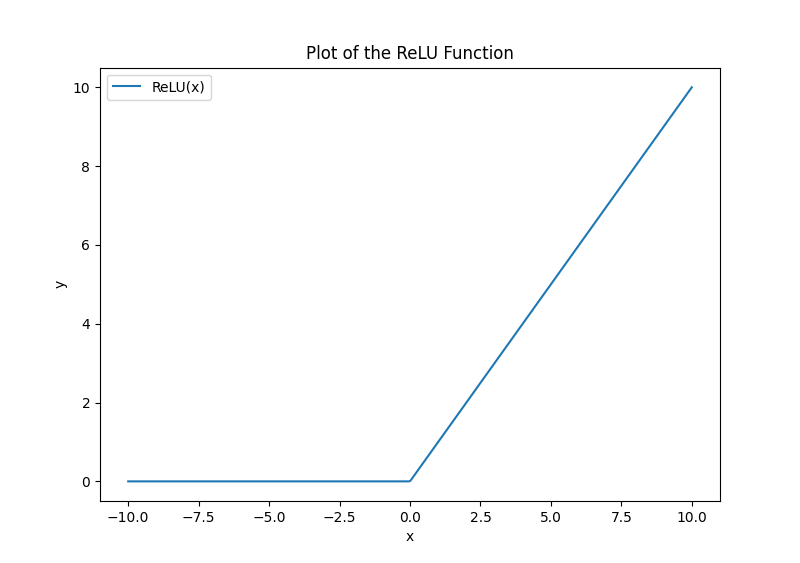
\includegraphics[width=80mm, height =50mm]{ReLU.png}
\end{frame}
\begin{frame}
	\frametitle{Leaky ReLU}
\center
	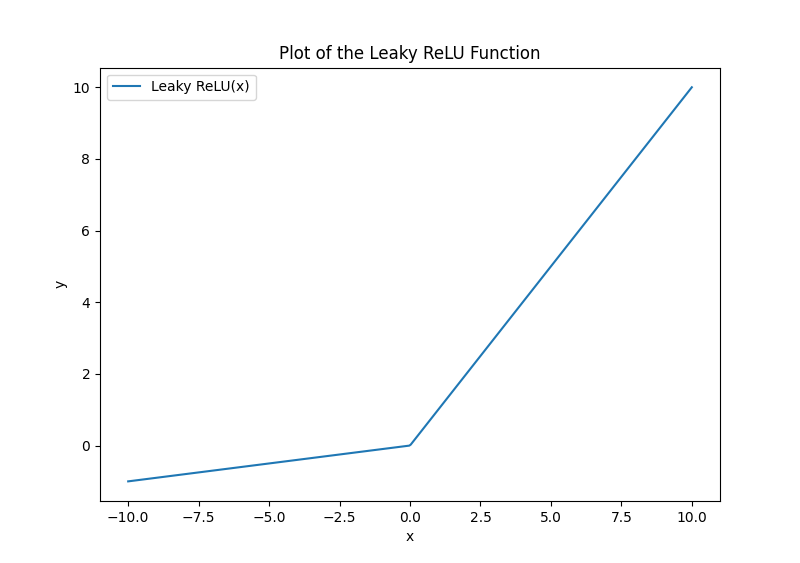
\includegraphics[width=80mm, height =50mm]{leaky_ReLU.png}
	
\end{frame}

\subsection{Logistic Sigmoid and Hyperbolic Tangent}
\begin{frame}
\frametitle{Logistic Sigmoid and Hyperbolic Tangent}
	\begin{itemize}
		\item Prior to the introduction of rectified linear units, most neural networks used the logistic sigmoid activation function
			$$g(z)= \sigma(z)$$
or the hyperbolic tangent activation function
			$$ g(z)= \tanh(z)$$
		\item $\tanh(z) = 2\sigma(2z)-1$
	\end{itemize}
\end{frame}
\begin{frame}
\begin{figure}[ht]
  \subcaptionbox{Logistic Sigmoid}[.50\linewidth]{%
    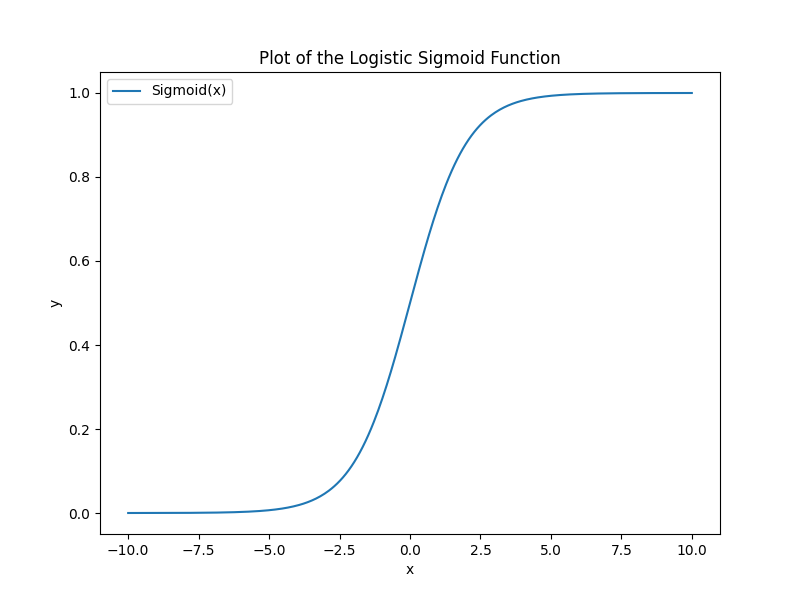
\includegraphics[width=\linewidth]{sigmoid.png}%
  }%
  \hfill
  \subcaptionbox{Hyperbolic Tangent}[.50\linewidth]{%
	  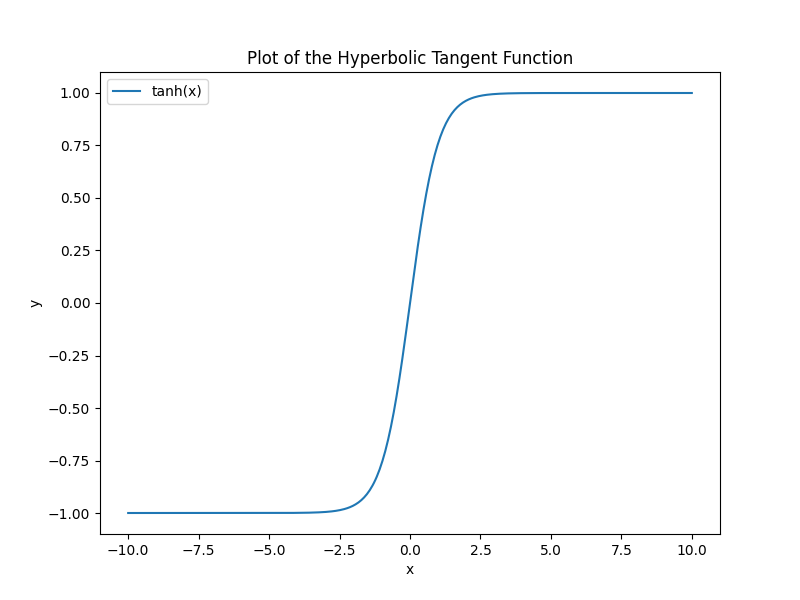
\includegraphics[width=\linewidth]{tanh.png}%
  }
\end{figure}

\end{frame}

\section{Architecture Design}
\begin{frame}
	\center 
	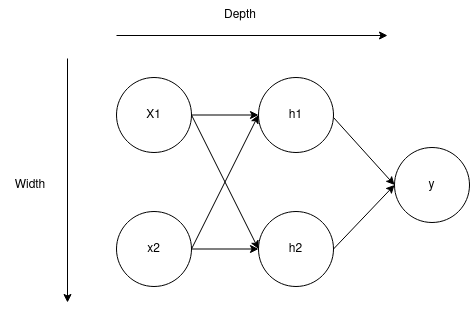
\includegraphics[width=110mm , height= 70mm]{width_depth.png}
	
\end{frame}
\begin{frame}
	\frametitle{What do we mean with architecture?}
	\begin{itemize}
		\item Architecture: the overall structure of the network: how many units it should have and how these units should be connected to each other
		\item Most neural network architectures arrange layers in a chain structure, with each layer being a function of the layer that preceded it
		\item The first layer is given by : 
			$$ h^{(1)} = g^{(1)}(W^{(1)T}x + b^{(1)})$$
		\item The second layer: 
			$$ h^{(2)} = g^{(2)}(W^{(2)T}x + b^{(2)})$$
		\item the main architectural considerations are choosing the depth of the network and the width of each layer
	\end{itemize}
\end{frame}
\begin{frame}
	\frametitle{The Universal Approximator Theorem}
	\begin{itemize}
		\item One hidden layer is enough to represent an approximation of any function to an arbitrary degree of accuracy
	\end{itemize}
	\center 
	So why deeper Networks?
	\begin{itemize}
		\item Shallow Network may need (exponentially) more width
		\item Shallow Network may overfit more
	\end{itemize}
\end{frame}
\begin{frame}
	\center 
	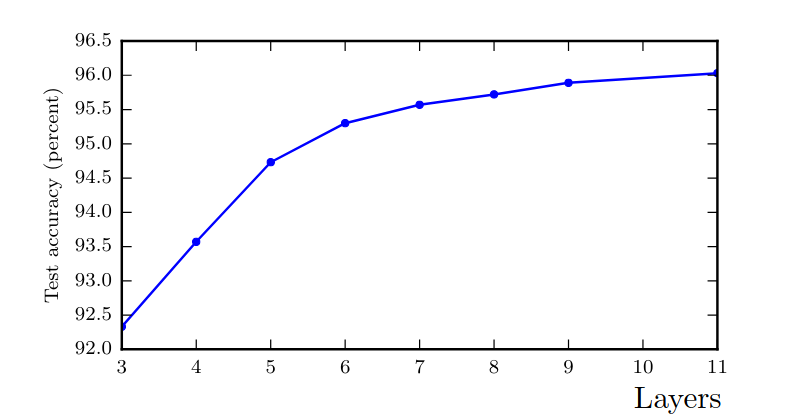
\includegraphics[width = 110mm , height= 60 mm]{depth_accuracy.png}
	
\end{frame}

\section{Back-Propagation}
\begin{frame}
	\frametitle{overview}
	\center
	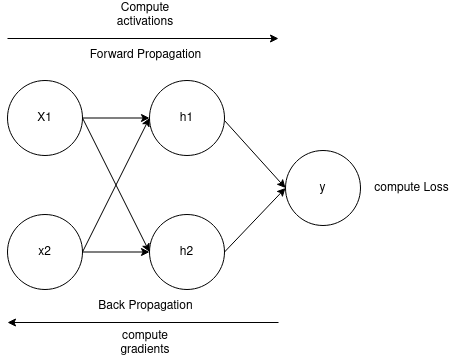
\includegraphics[width = 120mm , height = 70mm]{back_prop_graph.png}	
\end{frame}

\subsection{Computational Graphs}
\begin{frame}
	\begin{itemize}
		\item To describe the back-propagation Algorithm more precisely $\rightarrow$ a more precise computational Graph language
		\item each node indicates a variable(scalar, vector, matrix, tensor ...)
		\item Operation: a simple function of one or more variables
		\item a directed edge from x to y: y is computed by applying an operation to a variable x
		\item $\rightarrow$ just a way of expressing and evaluating a mathematical expression
	\end{itemize}
\end{frame}
\begin{frame}
	\frametitle{Example:}
	\center
	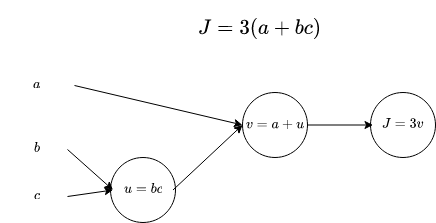
\includegraphics[width=100mm, height= 55mm]{comp_graph.png}
	
\end{frame}

\subsection{Chain Rule of Calculus}
\begin{frame}
	\frametitle{Chain Rule of Calculus}
\begin{itemize}
	\item used to compute the derivatives of functions formed by composing other functions
	\item Back-propagation is an algorithm that computes the chain rule, with a specific order of operations that is highly efficient
	\item Suppose that $y = g(x)$ and $z= f(g(x)) = f(y)$ then the chain rule states that: 
		$$ \frac{dz}{dx} = \frac{dz}{dy} \frac{dy}{dx}$$
	\item we can generalize this: $ x \in \mathbb{R}^m , y \in \mathbb{R}^n$ $g$ maps from $\mathbb{R}^m$ to $\mathbb{R}^n$ and $f$ from $\mathbb{R}^n$ to $\mathbb{R}$ then: 
		$$\nabla_{x}z = (\frac{\partial y}{\partial x})^T \nabla_{y}z $$
	\item $\frac{\partial y}{\partial x}$ is the $n \times m$ Jacobian matrix of $g$
\end{itemize}	
\end{frame}
\begin{frame}
	\frametitle{Recursively Applying the Chain Rule to obtain Backprop}
	\begin{itemize}
		\item Back-propagation is the chain rule of calculus recursively applied to compute gradients of expressions 
		\item It is a particular implementation of the chain rule
		\item uses dynamic programming (table filling) $\rightarrow$ to avoid recomputing repeated subexpressions
		\item Speed vs memory tradeoff
		
	\end{itemize}	
\end{frame}

\subsection{Back-propagation Computation}
\begin{frame}
	\frametitle{Repeated subexpressions}
	\begin{columns}
		\column{0.38\linewidth}
		\centering
		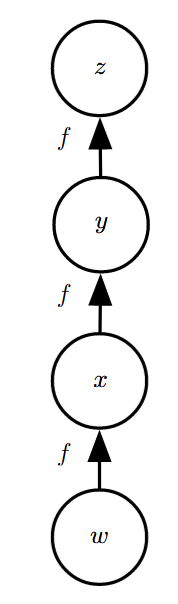
\includegraphics[height= 7cm, width = 3.5cm]{repeated_sub_exp.png}
		\column{0.58\linewidth}
		$$ \frac{\partial z}{\partial w}$$
		$$ = \frac{\partial z}{\partial y} \frac{\partial y}{\partial x} \frac{\partial x}{\partial w}  $$
		$$ = f'(y)f'(x)f'(w)$$
		$$ = f'(f(f(w)))f'(f(w))f'(w)$$
	\end{columns}

\end{frame}

\section{Historical Notes}
\begin{frame}
\frametitle{A Little History}
	\begin{chronology}[50]{1676}{2023}{60ex}[\textwidth]
	\event{1676}{The chain Rule of Calculus}

\end{chronology}
	\vspace{0.3cm}
	\begin{itemize}
		\item The chain rule that underlies the back-propagation algorithm was invented in the seventeenth century (Leibniz, 1676; L’Hôpital, 1696)
	\end{itemize}
\end{frame}
\begin{frame}
\frametitle{A little History}
\begin{chronology}[50]{1676}{2023}{60ex}[\textwidth]
	\event{1847}{Gradient Descent}

\end{chronology}
	\vspace{0.5cm}
	\begin{itemize}
	\item Gradient
descent was introduced as a technique for iteratively approximating the solution
to optimization problems in the nineteenth century (Cauchy, 1847).
	\end{itemize}
\end{frame}

\begin{frame}[t]
	\frametitle{A little History}
\begin{chronology}[50]{1676}{2023}{60ex}[\textwidth]
	\event{1940}{Linear Models}
\end{chronology}
	\begin{itemize}
			\vspace{1cm}
		\item Beginning in the 1940s, these function approximation techniques were used to motivate machine learning models such as the perceptron. However, the earliest models were based on linear models
	\end{itemize}
\end{frame}
\begin{frame}\frametitle{A little History}
\begin{chronology}[50]{1676}{2023}{60ex}[\textwidth]
	\event{1986}{Back-propagation}
\end{chronology}
	\vspace{0.5cm}
	\begin{itemize}
		\item the first successful experiments with back-propagation
	\end{itemize}
\end{frame}
\begin{frame}\frametitle{A little History}
\begin{chronology}[50]{1676}{2023}{60ex}[\textwidth]
	\event[1986]{2015}{improvements in NN performance}
\end{chronology}
	\vspace{0.5cm}
	\begin{itemize}
		\item Most of the improvement in neural
network performance from 1986 to 2015 can be attributed to the following factors
	\end{itemize}
\end{frame}
\begin{frame}
	\frametitle{Why is Deep Learning taking off?}
	\begin{itemize}
		\item larger dataset
		\item neural networks have become much larger,
because of more powerful computers and better software infrastructure
\item some algorithmic changes have also improved the performance of neural
networks noticeably
\item  the replacement of mean squared error
with the cross-entropy family of loss functions		
	\item the replacement of sigmoid hidden units with piecewise
linear hidden units, such as rectified linear units
	\end{itemize}
	
\end{frame}

\section{Code demo}
\begin{frame}
	\frametitle{Code demo}
\center 
Puting it together: Planar Data Classification
\end{frame}

\begin{frame}
	\center 
	Thank you
\end{frame}

\begin{frame}
\bibliographystyle{amsalpha}
\bibliography{presentation.bib}
\end{frame}
\end{document}
